% =============================================================================
% Chapter 5: System Architecture and Implementation
% =============================================================================

\chapter{System Architecture and Implementation}
\label{chap:system_architecture_implementation}

In this chapter, we present the system architecture and implementation of the semantic annotation platform. The architectural design prioritizes three fundamental principles: extensibility across various LLM providers, traceability of annotation decisions for auditability, and modularity to accommodate both batch experimentation and interactive analysis workflows.

% =============================================================================
% Section 5.1: System Overview
% =============================================================================

\section{System Overview}
\label{sec:system_overview}

% =============================================================================
% Section 5.2: Architecture
% =============================================================================

\subsection{Architecture}
\label{subsec:architecture}

We adopt a standard four-layer architecture, as illustrated in Figure~\ref{fig:system_overview}, to promote modularity and separation of concerns. The Web Interface enables user interaction and data visualization. The API Gateway serves as the communication bridge, handling request routing and command dispatching. Followed by the Core Engine, which encapsulates the primary computational modules, including data processing engine, the semantic annotation engine, and evaluation engine. Finally, the Data Storage manages the persistence of ontologies, tabular data, and system configurations. Architecturally, the system is deployed with a decoupled frontend and a unified backend service.

\begin{figure}[htbp]
    \centering
    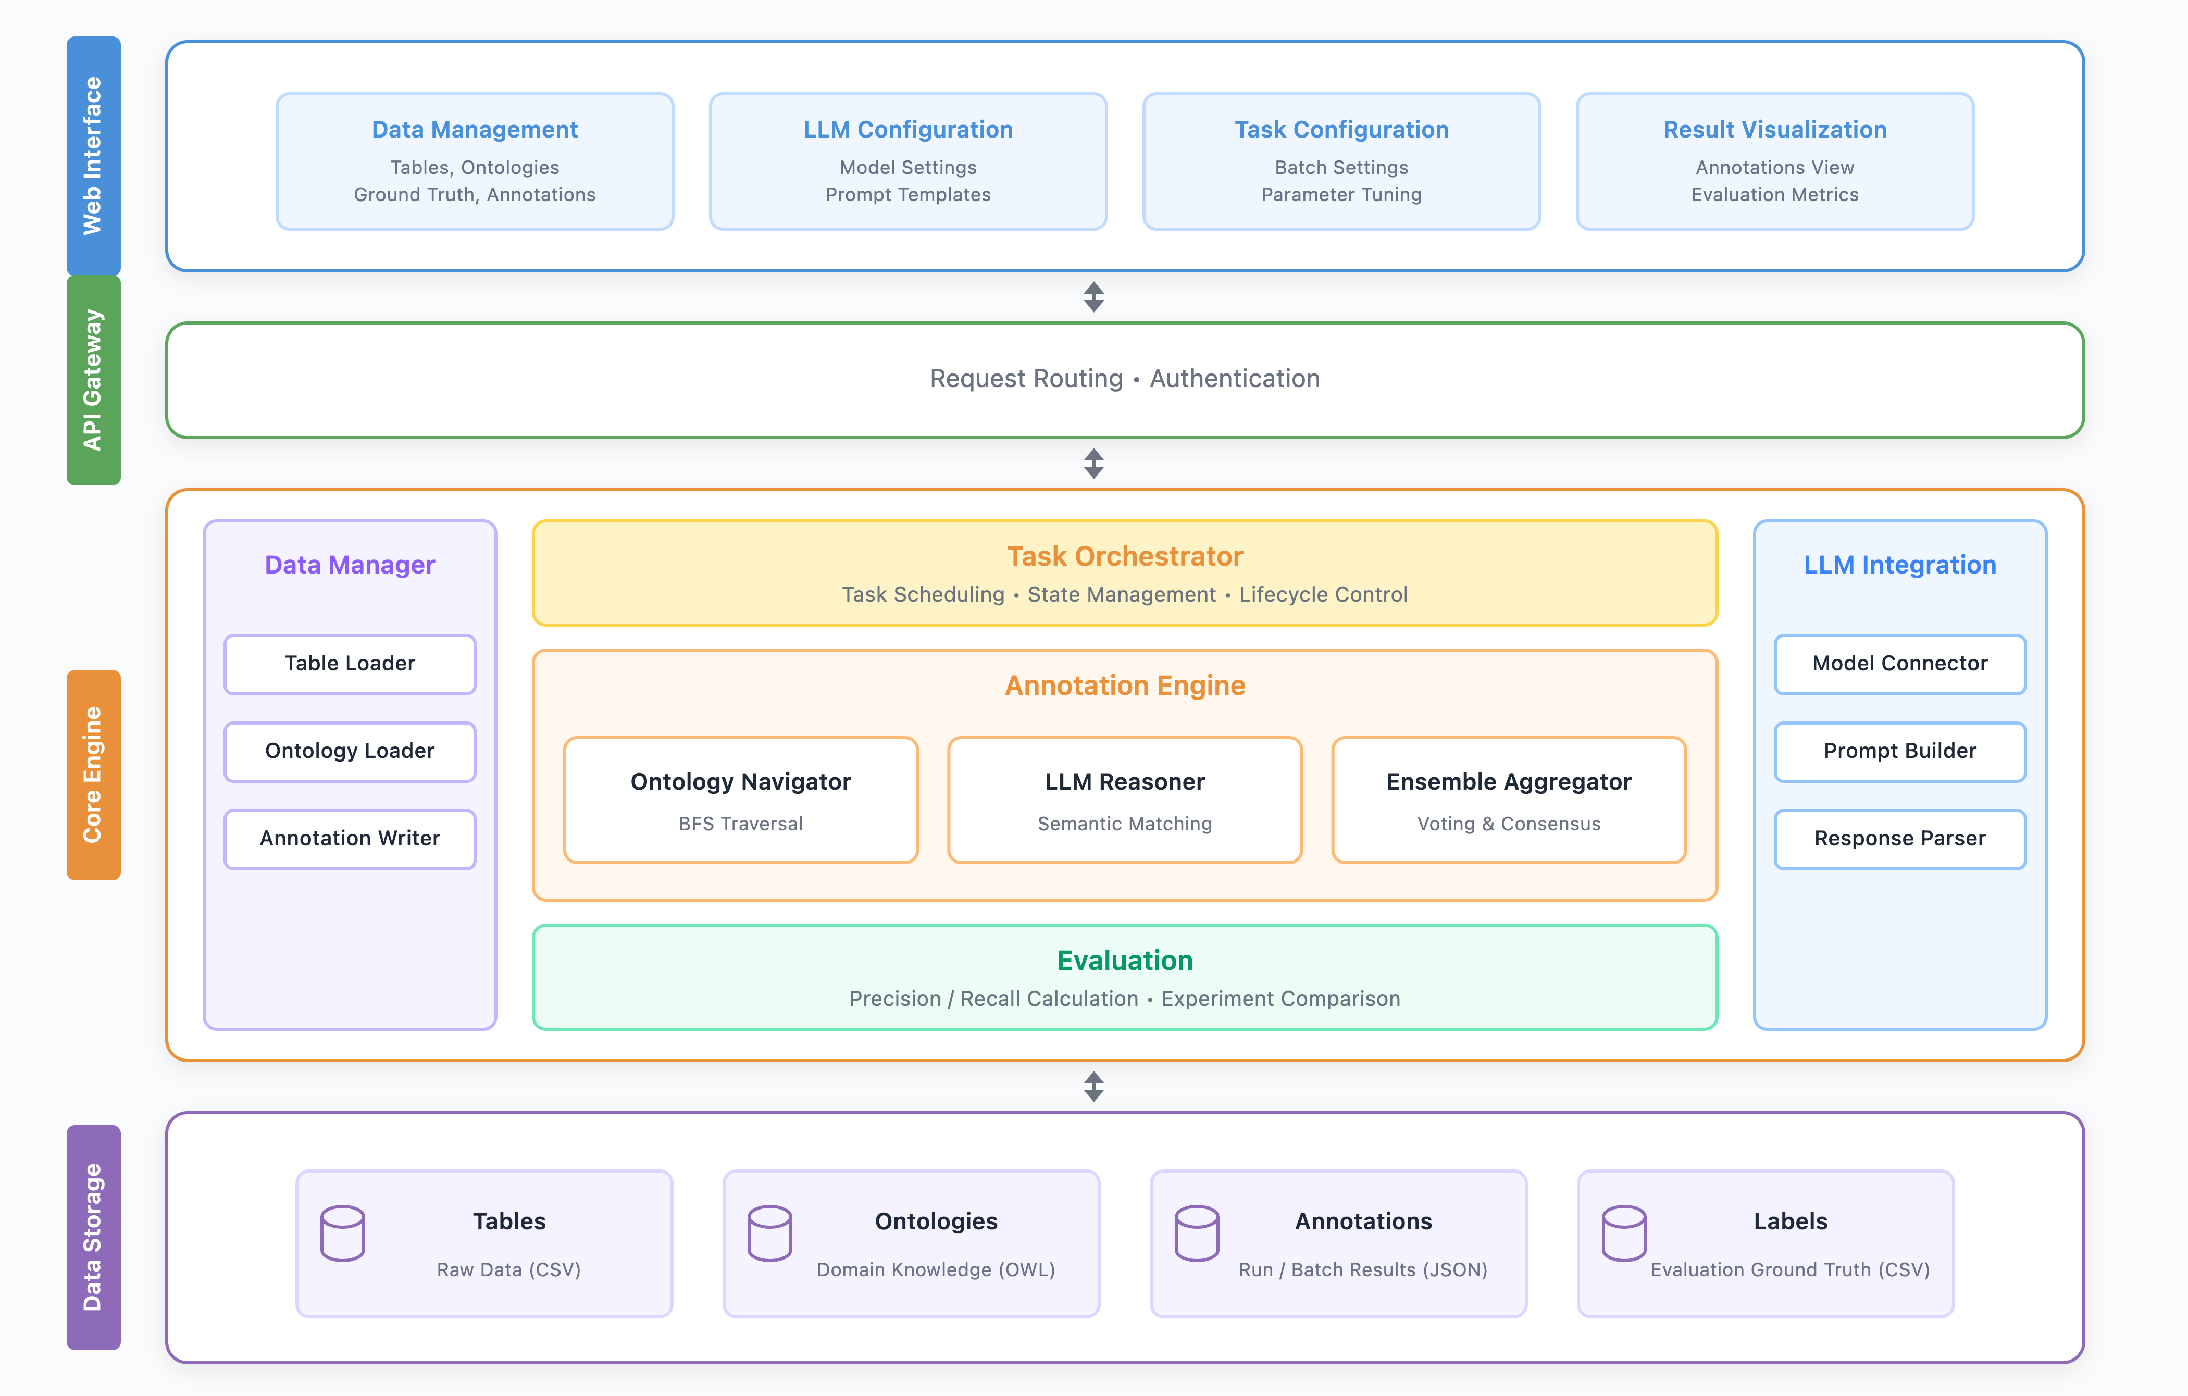
\includegraphics[width=\textwidth]{graphics/canvas/system_overview.pdf}
    \caption{System Architecture Overview. The architecture comprises four layers: Web Interface, API Gateway, Core Engine, and Data Layer. The Core Engine orchestrates the semantic annotation process through modules such as Task Orchestrator, Annotation Engine, and Evaluation.}
    \label{fig:system_overview}
\end{figure}

The architecture accommodates two complementary operational modes. \textbf{Interactive analysis} provides real-time monitoring and granular inspection of annotation decisions. Additionally, a Command Line Interface (CLI) provides additionaly a programmatic interface for \textbf{Batch processing} and automation, enabling high-throughput analysis across datasets and facilitating systematic empirical evaluation.

\subsection{Component Description}
\label{subsec:component_description}

The system architecture comprises four hierarchical layers, each encapsulating distinct functional responsibilities.

\paragraph{Web Interface.}
This layer exposes user-facing functionality through four modules: Data Management handles ingestion and organization of tables, ontologies, and ground truth artifacts; LLM Configuration manages model selection and prompt template specification; Task Configuration controls batch settings and algorithmic parameter tuning; Result Visualization renders annotations and evaluation metrics. Collectively, these modules constitute the primary interaction surface for end users.

\paragraph{API Gateway.}
This layer mediates request routing, concurrency management, and authentication. By abstracting communication between frontend and backend services, it ensures consistent request processing and decouples presentation logic from business logic.

\paragraph{Core Engine.}
This layer implements the primary computational logic through three integrated components. The Task Orchestrator manages scheduling, state transitions, and lifecycle control. The Annotation Engine comprises three submodules: the Ontology Navigator for hierarchical traversal, the LLM Reasoner for semantic matching, and the Ensemble Aggregator for vote consolidation. The Evaluation Module computes precision, recall, and related metrics against ground truth annotations. This layer represents the algorithmic core of the platform.

\paragraph{Data Layer.}
This layer persists four categories of artifacts: Tables containing raw input data, Ontologies encoding domain knowledge structures, Annotations storing run and batch results, and Ground Truth providing evaluation labels. This separation ensures referential integrity and supports reproducible experimentation.

\subsection{Data Flow}
\label{subsec:data_flow}

The annotation workflow adheres to a structured artifact lifecycle, ensuring traceability and reproducibility throughout execution.

\begin{enumerate}
    \item \textbf{Ontology Loading.} The ontology file undergoes parsing and transformation into a Directed Acyclic Graph (DAG) representation. The resulting artifact is registered with version metadata to ensure semantic stability across experiments.

    \item \textbf{Table Ingestion.} Input tables are parsed to produce Column Context objects encapsulating headers, type hints, and representative sample values. This normalization step isolates data heterogeneity from downstream annotation logic.

    \item \textbf{Annotation Execution.} The Breadth-first Search (BFS) executor traverses the ontology hierarchy, invoking the Ensemble Decision Making (EDM) module at each depth level to filter candidate classes. When multiple branches survive traversal, path selection is determined by accumulated branch scores.

    \item \textbf{Result Persistence.} Predictions are serialized alongside comprehensive execution traces capturing prompts, responses, and intermediate decisions. This linkage enables post-hoc analysis and error attribution.

    \item \textbf{Evaluation.} The evaluation module computes performance metrics by comparing predictions against ground truth annotations, generating the summary statistics requisite for empirical benchmarking.
\end{enumerate}

% =============================================================================
% Section 5.2: Core Components
% =============================================================================

\section{Core Components}
\label{sec:core_components}

\subsection{Ontology Management}
\label{subsec:ontology_management}

The Ontology Management module transforms static ontology artifacts into an optimized internal representation that facilitates efficient querying during annotation.

\paragraph{Loading and Parsing.}
The platform supports standard Semantic Web serializations, including RDF/XML and Turtle formats and OWL 2.0. During ingestion, the parser systematically extracts classes identified by Internationalized Resource Identifiers (IRIs), human-readable labels and descriptions, and hierarchical relationships based on the \texttt{rdfs:subClassOf} relation. Notably, anonymous classes and complex OWL restrictions are explicitly filtered to maintain a strict DAG structure comprising only named classes, which reduces computational complexity while preserving the taxonomic backbone essential for traversal.

\paragraph{DAG Construction and Caching.}
Following parsing, the ontology is formalized as a directed acyclic graph (DAG) $G=(V,E)$, where edge $(u,v) \in E$ indicates that $v$ is a subclass of $u$. To support efficient traversal, the system materializes two adjacency caches:
\begin{itemize}
    \item \textbf{Children Cache:} $\text{children}[u] = \{ v \mid (u,v) \in E \}$
    \item \textbf{Parents Cache:} $\text{parents}[v] = \{ u \mid (u,v) \in E \}$
\end{itemize}

The platform designates \texttt{owl:Thing} as the unique traversal root, ensuring consistency with standard OWL semantics. Furthermore, the DAG construction phase enforces structural integrity through active cycle detection. Although subclass relations are semantically intended to be acyclic, modeling errors occasionally introduce cycles that would cause infinite loops during traversal. When detected, cycles are resolved deterministically by pruning the edge that completes the cycle, thereby guaranteeing the DAG property required for BFS termination.

\subsection{Table Processing}
\label{subsec:table_processing}

The Table Processing module serves as the intermediary between raw tabular inputs and the annotation engine, producing compact, LLM-ready representations.

\paragraph{Input Formats and Parsing.}
The platform supports standard domain table formats, including CSV and Excel exports. The parser converts files into an internal dataframe representation preserving column headers as raw strings, cell values with explicit handling of missing data, and fundamental schema metadata. Given that domain tables frequently exhibit inconsistent encodings, such as mixed numeric and string fields or sentinel values, the parsing logic prioritizes robustness over strict type enforcement. When type inference is ambiguous, the system defaults to a mixed object type, delegating semantic disambiguation to the downstream LLM.

\paragraph{Column Context Extraction.}
For each column $c_i$, the module constructs a Column Context Object comprising three elements:
\begin{description}
    \item[Header:] The original column name, serving as the primary semantic signal.
    \item[Type Hint:] A coarse data type category (Numeric, Categorical, Timestamp, Boolean, or Mixed) derived through heuristic inference.
    \item[Sample Values:] A bounded set of representative values selected according to a configurable sampling policy.
\end{description}

The sampling step addresses a critical constraint: domain tables often contain extensive time series, rendering full-column inclusion token-prohibitive. Consequently, the platform enforces a hard cap on sampled values per column and applies consistent filtering rules to exclude nulls and whitespace, providing sufficient evidence for semantic disambiguation while maintaining predictable token consumption.

\paragraph{Batch Processing Support.}
The module provides batch-oriented utilities essential for dataset-scale experiments. These include dataset ingestion across table collections, progress reporting via the unified API, failure isolation to prevent individual parsing errors from aborting entire experiments, and deterministic outputs guaranteeing bit-identical context objects across repeated executions. This determinism constitutes a prerequisite for controlled comparative experiments.

\subsection{Annotation Engine}
\label{subsec:annotation_engine}

The Annotation Engine serves as the operational core executing the workflow. It orchestrates interactions among the ontology DAG, column contexts, and the LLM client abstraction layer.

\paragraph{Execution Workflow.}
At runtime, the engine adheres to a deterministic execution protocol. First, it initializes the run context by loading the target ontology snapshot structurally rooted at \texttt{owl:Thing}. Subsequently, for each column, the engine initiates traversal at the root and iterates level-by-level: valid child nodes are retrieved via the children cache, the EDM module evaluates the candidate set and returns survivors, and new branches are enqueued for expansion. Traversal terminates when no survivors remain or the configured depth limit is reached. Finally, when multiple branches survive, the engine selects the optimal path based on the highest accumulated branch score. Given fixed inputs and deterministic provider behavior, the control flow remains strictly reproducible.

\paragraph{Result Caching.}
To mitigate redundant computation during iterative experimentation, the engine implements caching at the final result level, mapping configurations to predicted paths. However, cache reuse is strictly validated: results are deemed reusable only when the ontology snapshot, prompt template identifier, model provider settings, and EDM parameters match the current configuration exactly.

\paragraph{Error Handling and Retry Logic.}
Given the engine's dependency on external LLM APIs, robust error handling is fundamental. The executor encapsulates provider interactions within a reliability layer featuring exception capture for request-level failures, exponential backoff strategies for transient errors, and graceful degradation that records failures in the execution trace rather than aborting the entire annotation run. All exceptions are logged with precise timestamps and provider identifiers, facilitating diagnosis of partial failures in runs involving hundreds of API calls.

\subsection{Evaluation Module}
\label{subsec:evaluation_module}

The Evaluation Module performs systematic assessment by computing node-level and path-level metrics against ground truth annotations. Specifically, it calculates precision, recall, and F1 scores, aggregating results across datasets. By integrating evaluation as a first-class pipeline component, the system ensures that experimental results remain reproducible and directly comparable.

% =============================================================================
% Section 5.3: Traceability and Observability
% =============================================================================

\section{Traceability and Observability}
\label{sec:traceability}

A central design tenet of the platform is that annotation results must not be treated as opaque outputs; rather, they constitute verifiable decisions subject to inspection, reproduction, and audit. Since the system relies on external LLM providers and stochastic inference, traceability is implemented as a first-class concern.

\subsection{Execution Logging}
\label{subsec:execution_logging}

For each column and at every BFS depth level, the system persists a granular log entry capturing five dimensions:
\begin{itemize}
    \item \textbf{Context:} The column identifier and its extracted context (name, type, samples).
    \item \textbf{State:} The set of candidate ontology classes considered at that level.
    \item \textbf{Decisions:} The EDM outcomes, including vote counts, selected survivors, and support scores.
    \item \textbf{Evidence:} The verbatim prompts transmitted to the provider and raw responses received.
    \item \textbf{Metadata:} Operational metrics including request latency.
\end{itemize}

Notably, token usage data is recorded only when explicitly provided by the runtime. If the provider does not return usage statistics, the field is recorded as null. This policy prevents conflation of precise provider-reported costs with local approximations, ensuring data integrity for downstream cost analyses.

\subsection{Real-Time Monitoring}
\label{subsec:real_time_monitoring}

Long-running annotation tasks expose their state via Server-Sent Events (SSE). The executor streams structured events including:
\begin{itemize}
    \item \textbf{Progress:} Current completion status (processed columns versus total).
    \item \textbf{Intermediate Results:} Predicted paths for columns immediately upon completion.
    \item \textbf{Operational Status:} Warnings, errors, and retry notifications.
    \item \textbf{Completion Summaries:} Aggregate runtime metrics and final status.
\end{itemize}

This streaming architecture enables the Web UI to reflect system behavior dynamically without polling. Consequently, users can identify configuration issues---such as overly strict thresholds yielding empty selections---while jobs remain in progress. This immediate feedback loop significantly accelerates iterative refinement.

% =============================================================================
% Section 5.4: Implementation Details
% =============================================================================

\section{Implementation Details}
\label{sec:implementation}

\subsection{Technology Stack}
\label{subsec:technology_stack}

\paragraph{Backend Infrastructure.}
The backend logic is implemented in Python, selected for its dominant ecosystem in data processing, semantic web tooling (e.g., \texttt{rdflib}), and machine learning integration. The system exposes functionality through an asynchronous web service built upon FastAPI, which provides strict schema validation via Pydantic models, native support for asynchronous concurrency enabling long-running jobs and real-time SSE streaming, and ASGI compliance facilitating deployment across diverse environments.

\paragraph{Frontend Interface.}
The interactive user interface is constructed using Next.js, a React-based framework enabling a modern single-page application experience. The frontend manages configuration workflows, provides real-time observability via SSE subscription, and offers specialized views for auditing intermediate decisions.

\paragraph{Data Persistence.}
To support auditability and portability, the platform adopts a lightweight persistence model centered on a file-based JSON Registry. Rather than relying on a database management system, key artifacts are persisted as structured files. The registry manages ontology snapshots with unique identifiers and parsing statistics, dataset configurations recording file paths and normalization rules, experiment manifests capturing provider settings and EDM parameters, and execution traces containing full logs of prompts, responses, and latency. The file-centric approach facilitates easy export and sharing of experimental data, enabling researchers to reproduce results independent of the original runtime environment.

\subsection{User Interfaces}
\label{subsec:user_interfaces}

\subsubsection{Command-Line Interface}
\label{subsubsec:cli}

The Command-Line Interface (CLI) serves as a robust control layer designed to facilitate reproducible experimentation and automated workflow orchestration.
In contrast to manual execution, the CLI enables precise configuration of the semantic annotation lifecycle through a modular command structure.
The system exposes three primary directives:

\begin{itemize}
    \item \textbf{Annotation Execution:} \\ 
    \texttt{saed-run --table --ontology --mode --output-dir} \\
    Initiates the annotation process for a single table, supporting detailed configuration of the reasoning mode and prompt strategy.
    \item \textbf{Batch Processing:} \\
    \texttt{saed-run-batch --config batch.yaml} \\
    Orchestrates parallel execution across multiple datasets, enabling systematic comparative experiments defined via declarative configuration files.
    \item \textbf{Evaluation:} \\
    \texttt{saed-eval <batch\_file> --labels <ground\_truth> --format all} \\
    Computes comprehensive performance metrics, including node-level and path-level precision, recall, and F1 scores.
\end{itemize}

The system employs a file-system-based synchronization mechanism for Ontology and Dataset registries, eliminating the need for explicit registration commands.
Table~\ref{tab:cli_parameters} strictly defines the configurable parameters for the execution runtime.

\begin{table}[htbp]
    \centering
    \caption{Key CLI parameters for the execution runtime.}
    \label{tab:cli_parameters}
    \renewcommand{\arraystretch}{1.2}
    \small
    \begin{tabular}{lp{3cm}p{7cm}}
        \toprule
        \textbf{Parameter} & \textbf{Category} & \textbf{Description} \\
        \midrule
        \texttt{--table}      & Data      & Registry ID or filename of the target table \\
        \texttt{--ontology}   & Data      & Registry ID or filename of the domain ontology \\
        \texttt{--mode}       & Algorithm & Decision mode (\texttt{single} or \texttt{edm}) \\
        \texttt{--max\_depth} & Algorithm & Maximum traversal depth for the BFS strategy \\
        \texttt{--provider}   & Model     & LLM backend service (overrides config) \\
        \texttt{--output-dir} & System    & Directory path for persisting run artifacts \\
        \bottomrule
    \end{tabular}
\end{table}

This architecture ensures that all experiments are idempotent and fully reproducible.
The batch processor further supports shell-level orchestration, facilitating the migration of experimental setups between diverse computational environments while respecting provider rate limits.

\subsubsection{Web Interface}
\label{subsubsec:web_interface}

While the CLI optimizes for high-throughput batch experimentation, the Web Interface addresses the complementary requirement for interactive execution and granular inspection. The graphical interface enables researchers to scrutinize decision boundaries and trace reasoning paths for specific column mappings, supporting seamless transition between parameter tuning and validation.

\subsection{API Design}
\label{subsec:api_design}

The platform exposes its core functionality through a compact HTTP API, employing two distinct interaction paradigms to balance control and observability.

\paragraph{RESTful Endpoints.}
The REST API adheres to a resource-oriented design philosophy, minimizing client-side complexity while providing full access to the system's capabilities:
\begin{itemize}
    \item \texttt{POST /api/runs} -- Submit a new annotation job. Returns a unique run identifier upon successful initialization.
    \item \texttt{GET /api/runs/\{run\_id\}} -- Query the current status, progress counters, and configuration metadata of a specific run.
    \item \texttt{POST /api/evaluations} -- Compute performance metrics for a completed batch against ground truth references.
    \item \texttt{GET /api/evaluations/compare} -- Comparative analysis of multiple runs to benchmark different configurations.
\end{itemize}

\paragraph{Real-Time Streaming via SSE.}
For long-running annotation tasks, polling REST endpoints introduces unnecessary latency and inefficiency.
Therefore, the backend exposes a dedicated streaming endpoint \texttt{GET /api/runs/\{run\_id\}/stream}, emitting structured JSON events conforming to the \texttt{text/event-stream} content type.
Events include fine-grained progress updates (e.g., \texttt{column\_start}, \texttt{step}), intermediate results, and completion summaries.

Server-Sent Events (SSE) were selected over WebSockets due to their lightweight implementation profile and native browser support for unidirectional server-to-client updates.
This design aligns with the annotation execution model, where the client primarily consumes status updates.
Combined with comprehensive execution logging, this API architecture ensures robust observability, enabling users to initiate jobs programmatically via REST and monitor their evolution in real-time.


